\chapter{Backend Mystery} 
Teakwood is powered by Django framework, so its backend inherits all the Django  feathers. For example, Teakwood follows the MVC(Model-View-Controller) design pattern and DRY(Don't Repeat Yourself) principle. When you go through Teakwood's code, you will found that teakwood have a neat and loose coupling coding structure. In this chapter, I will go through some most special feathers in the backend of Teakwood. I will use some Django terminologies for elaboration, If you want a better under standing of Django terminologies, please refer to the Django official documentations.

\section{MTV Framework}
Teakwood has an updated MVC, that is MTV.\\
\begin{figure}[htb]
\centering
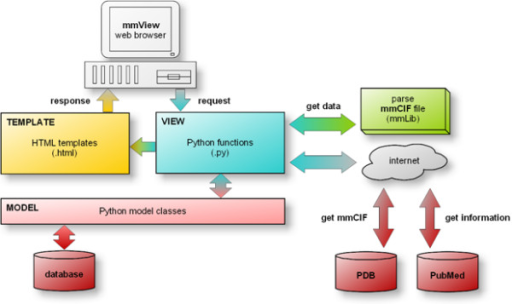
\includegraphics[scale=0.5]{./mtv}
\caption{Teakwood MTV framework}
\label{fig:label} % insert suitable label, this is used to refer to a fig from within the text as shown above
\end{figure}

\textbf{M} represents the model (Model), i.e., \textbf{the data access layer}. This layer processing data in all matters related to: how to access, how to confirm the validity , which behaviors it has, and the relationships between the data.\\
\textbf{T} Representative of T template (Template), i.e., \textbf{the presentation layer}. The layer processing performance related decision: how to display the page or other types of documents.\\
\textbf{V} represents the view (View), \textbf{business logic layer}. This layer contains the access models and the transfer of appropriate template logic. You can see it as a bridge between the model and the template.\\
\section{Models and Database}
Django provides an abstraction layer (the “models”) for structuring and manipulating the data of your Web application. In Django, a lot of this hassle is taken care of for you by Django’s object relational mapping (ORM) functions, and how Django encapsulates databases tables through models. Essentially, a model is a Python object that describes your data model/table. Instead of directly working on the database table via SQL, all you have to do is manipulate the corresponding Python object. 
\section{Teakwood Template Language}
Django’s template language is designed to strike a balance between power and ease. Its designed to feel comfortable to those used to working with HTML. \\
Django template language is not just HTML file. Here is an example:
\begin{verbatim}

{{ section.title }}

<h1>{{ section.title }}</h1>

<h2>
  <a href="{{ story.get_absolute_url }}">
    {{ story.headline|upper }}
  </a>
</h2>
<p>{{ story.tease|truncatewords:"100" }}</p>


\end{verbatim}

\textbf{Variable}: When the template engine encounters a variable, it evaluates that variable and replaces it with the result.\\

\textbf{Tag }: Tags are more complex than variables: Some create text in the output, some control flow by performing loops or logic, and some load external information into the template to be used by later variables. Some tags require beginning and ending tags. There are about two dozens of build-in tags in Django.\\

\textbf{filter}:Filter is basically a restricted variable.\\

we can add variables,tags and filters into HTML code.

\section{Powerful Admin}
Teakwood comes with a user authentication system which is inherited from Django framework. The admin system handles user accounts, groups, permissions and cookie-based user sessions. This section of the documentation explains how the default implementation works out of the box, as well as how to extend and customize it to suit your project needs.

Teakwood Admin system limited to trusted site administrators, that enables the adding, editing and deletion of site content. Some common examples: the interface you use to post to your blog, the backend site managers use to moderate user-generated comments, the tool your clients use to update the press releases on the Web site you built for them.

\section{A Practical Case}

How Teakwood process a request from user?
\begin{figure}[htb]
\centering
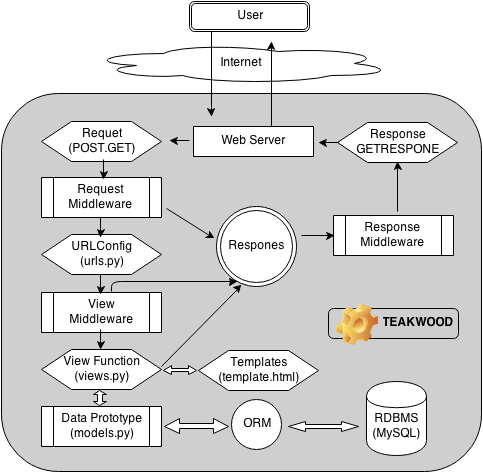
\includegraphics[scale=0.6]{./http_request_response}
\caption{Teakwood Request-Response Working Flow}
\label{fig:label} % insert suitable label, this is used to refer to a fig from within the text as shown above
\end{figure}

%\section{Lose Coupling}


